\section{Particle Kinetics}

\subsection{Classical mechanics}
\blue{Complete in "Kinetics of point masses"}
    \subsubsection{Method of assumed forces and method of assumed motion}
    \blue{Complete in "Kinetics of point masses"}
    \subsubsection{Solution steps}
    \blue{Complete in "Kinetics of point masses"}
    \blue{More information about Free body diagrams included in "Free boy diagrams"}

\subsection{\red{Numerical integration}}

\red{Add information shown in Fig \ref{fig:NumericalIntegration}}

\begin{figure}[h!]
    \centering 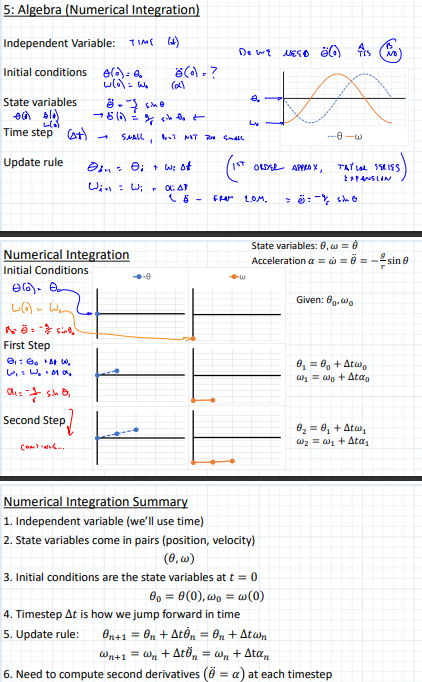
\includegraphics{ParticleKinetics/NumericalIntegration.png}
    \caption{From L14-Notes, slides 7-9}
    \label{fig:NumericalIntegration}
\end{figure}

\subsection{\red{Applications}}
    \subsubsection{\red{Kiiking}}
    \red{This topic is in L13-Notes, slides 9-10. Include information in Fig \ref{} and this YouTube link \url{https://www.youtube.com/shorts/qvW0sz4kBLQ}}. Application for "Particle kinetics".

    \begin{figure}[h!]
        \centering
        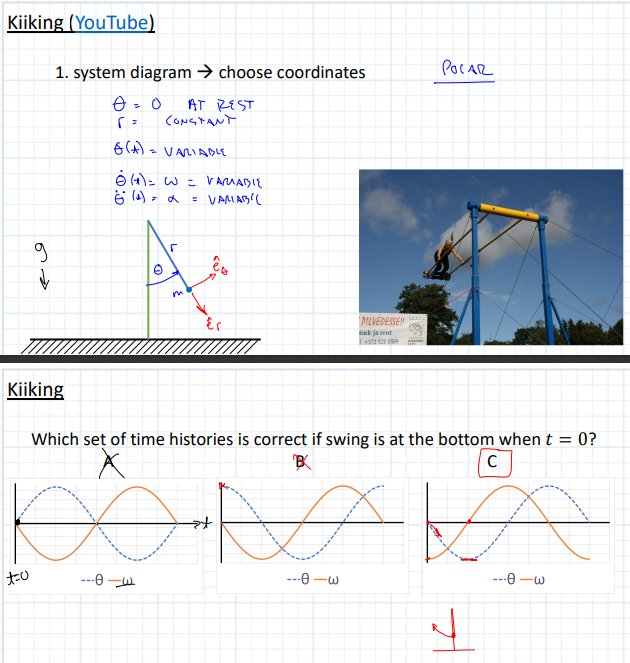
\includegraphics{ParticleKinetics/AppKiiking.png}
        \caption{From L13-Notes, slides 9-10.}
        \label{fig:AppKiiking}
    \end{figure}

    \subsubsection{Accelerating and braking}
    \label{sub:PartKin_acce}
    \blue{Complete in "Accelerating and braking". Just the introduction and the information under "Point mass model".} 

    \subsubsection{Banked turns}
    \label{sub:PartKin_turns}
    \blue{Complete in "Banked turns". Just the introduction and the information under "Track geometry" and "Point mass model".} 

    \subsubsection{Projectiles with air resistance}
    \blue{Complete in "Projectiles with air resistance".} 